\section{Задание}

Создать схему, имитирующую работу трёх СЗИ для защиты от трёх независимых типов атак. 

Для первого типа атак СЗИ1 – основной, СЗИ2 – резервный. Для второго типа атак СЗИ2 – основной, СЗИ3 – резервный. Для третьего типа атак СЗИ3 – основной, СЗИ1 – резервный. 

Для первого типа атак generate = 30, для второго типа атак generate = 25, для третьего типа атак generate = 20. 

СЗИ1 имеет advance = 25, СЗИ2 имеет advance = 20, СЗИ3 имеет advance = 25. 

Показать загрузку очередей, процент отражённых и прошедших атак каждого типа и по каждому СЗИ. 

Количество атак – 10000.

\section{Ход работы}

Код для моделирования в среде GPSS представлен ниже:

\begin{Verbatim}[frame=single,fontsize=\small]
; ПЕРВЫЙ ТИП АТАК: СЗИ1 - ОСНОВНОЙ, СЗИ2 - РЕЗЕРВНЫЙ; GENERATE = 30
; ВТОРОЙ ТИП АТАК: СЗИ2 - ОСНОВНОЙ, СЗИ3 - РЕЗЕРВНЫЙ; GENERATE = 25 
; ТРЕТИЙ ТИП АТАК: СЗИ3 - ОСНОВНОЙ, СЗИ1 - РЕЗЕРВНЫЙ; GENERATE = 20
; СЗИ1: ADVANCE = 25; СЗИ2: ADVANCE = 20; СЗИ3: ADVANCE = 25
; КОЛИЧЕСТВО АТАК = 10000

    GENERATE 30 ; ПЕРВЫЙ ТИП АТАК
SZI1_GENERAL TEST LE Q$QUEUE1,1,SZI1_RESERV ; СЗИ1 - ОСНОВНОЙ
    QUEUE QUEUE1
    SEIZE CHANNEL1
    DEPART QUEUE1
    ADVANCE 25,1
    RELEASE CHANNEL1
    TRANSFER ,SZI1_FAIL
SZI1_RESERV TEST LE Q$QUEUE2,1,SZI1_FAIL; СЗИ2 - РЕЗЕРВ ДЛЯ СЗИ1
    QUEUE QUEUE2
    SEIZE CHANNEL2
    DEPART QUEUE2
    ADVANCE 20,1
    RELEASE CHANNEL2
SZI1_FAIL TERMINATE 1

    GENERATE 25; ВТОРОЙ ТИП АТАК
SZI2_GENERAL TEST LE Q$QUEUE2,1,SZI2_RESERV ; СЗИ2 - ОСНОВНОЙ
    QUEUE QUEUE2
    SEIZE CHANNEL2
    DEPART QUEUE2
    ADVANCE 20,1
    RELEASE CHANNEL2
    TRANSFER ,SZI2_FAIL
SZI2_RESERV TEST LE Q$QUEUE3,1,SZI2_FAIL; СЗИ3 - РЕЗЕРВ ДЛЯ СЗИ2
    QUEUE QUEUE3
    SEIZE CHANNEL3
    DEPART QUEUE3
    ADVANCE 25,1
    RELEASE CHANNEL3
SZI2_FAIL TERMINATE 1

   GENERATE 20; ТРЕТИЙ ТИП АТАК
SZI3_GENERAL TEST LE Q$QUEUE3,1,SZI3_RESERV ; СЗИ3 - ОСНОВНОЙ
    QUEUE QUEUE3
    SEIZE CHANNEL3
    DEPART QUEUE3
    ADVANCE 25,1
    RELEASE CHANNEL3
    TRANSFER ,SZI3_FAIL
SZI3_RESERV TEST LE Q$QUEUE1,1,SZI3_FAIL; СЗИ1 - РЕЗЕРВ ДЛЯ СЗИ3
    QUEUE QUEUE1
    SEIZE CHANNEL1
    DEPART QUEUE1
    ADVANCE 25,1
    RELEASE CHANNEL1
SZI3_FAIL TERMINATE 1

    START 10000
\end{Verbatim}

~\\

Статистика по блокам моделирования представлена на рисунке 1.

\begin{figure}[ht!]
    \centering
    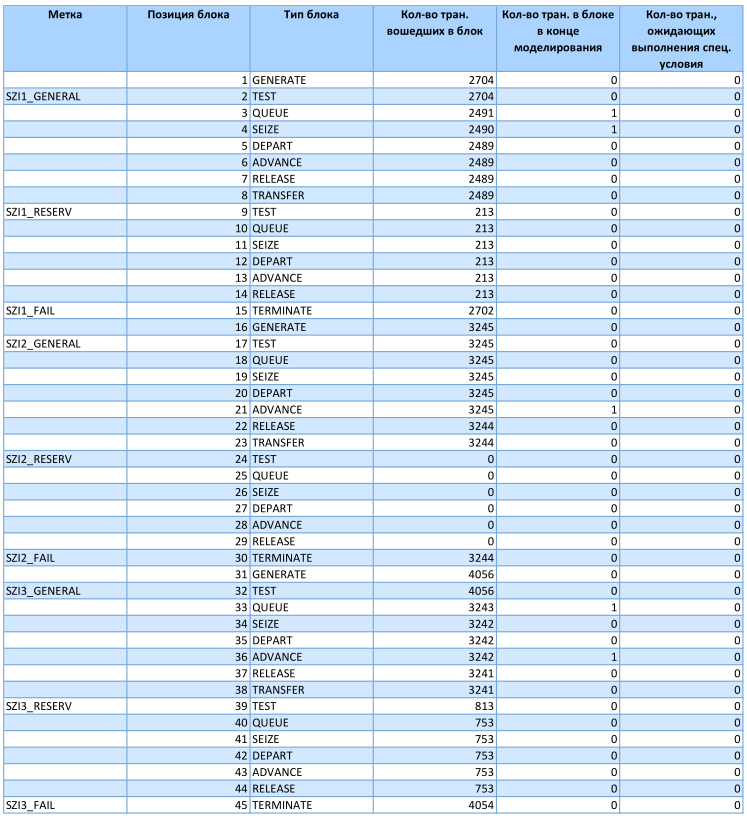
\includegraphics[width=\textwidth]{inc/blocks}
    \caption{Статистика моделирования}
\end{figure}

~\\

На основании этих статистичнских данных можно построить дианграммы отражения атак. Анализ загрузки СЗИ представлен на рисунке 2.

\begin{figure}[ht!]
    \centering
    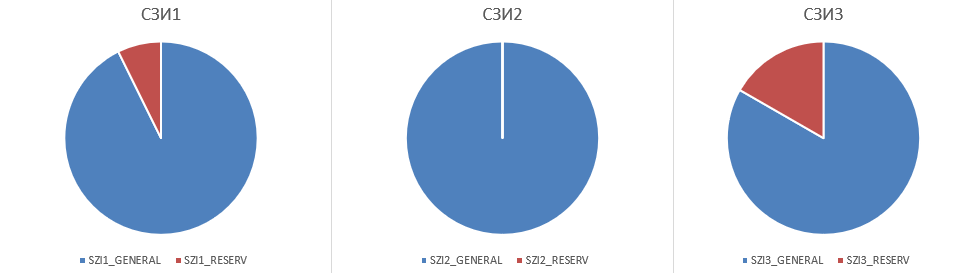
\includegraphics[width=0.9\textwidth]{inc/diag}
    \caption{Диаграмма загрузки СЗИ}
\end{figure}

Из диаграммы видно, что часть СЗИ1 перешло на резевное СЗИ2 при полной загрузке СЗИ1. СЗИ2 полность справилось с атаками. Часть атак СЗИ3 была отражена резервным СЗИ1 при полной загрузке СЗИ3.

\section{Выводы}

Рассмотрена система моделирования GPSS, построена модель СЗИ (схема из трёх СЗИ), проведён анализ отражённых СЗИ атак. 